\section{Language Overview}
\label{sec:Overview}

\begin{figure}
  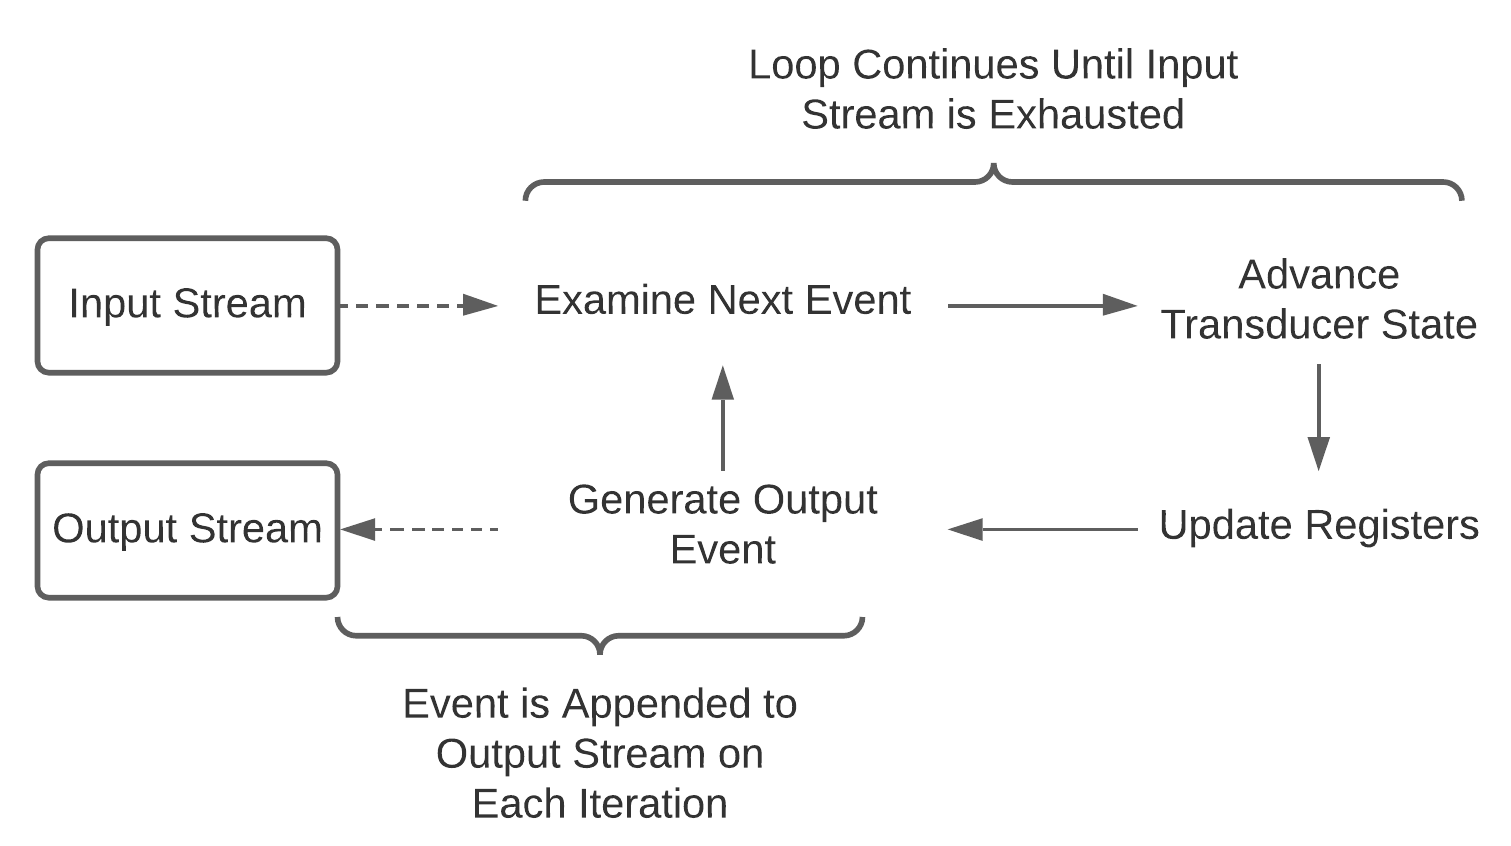
\includegraphics[scale=.8]{images/processing}
  \caption{A mutator individually processes each item in an input
  sequence, updating it's internal state and producing output according
  to the rules described in its program.}
  \label{fig:Processing}
\end{figure}

\preston{The processing figure is not mentioned anywhere}

The purpose
of a CSlang program is to completely describe a mutator
that both
accepts a chosen stream if it contains a particular
activity sequence and can produce a modified
output stream
for application testing.
Because a mutator is essentially a
transducer enhanced to operate over complex data structures
rather than symbols in a string
this description must cover all states,
the associated output of those states,
and the transition
relation that ties them all together.
Simply enumerating every aspect of a mutator could be very verbose
so we intentionally tailored CSlang's semantics to allow its users to
describe complex configurations in a concise manner.
In this Section we cover the design decisions we made
in of this goal.
Section~\ref{sub:ProcessingEventStreams} describes how executing a program works
while
in Sections~\ref{sub:PreambleAndBody}~and~\ref{sub:SyntaxAndSemantics},
we discuss the
language's syntax and semantics and illustrate the details
of these properties
with small examples.
Section~\ref{sub:DatawordOperators} takes a more
detailed look at important operators.

\subsection{Processing and Event Streams}
\label{sub:ProcessingEventStreams}
CSlang was written to
apply event processing
techniques to application activity
in order to catch bugs and drive further
testing.
To accomplish this, a CSlang program maps this activity onto an
event stream
made up of a chronological listing of the function calls, library
calls, system calls, or other structured requests made by the program.
Within this stream each element consists of two pieces: a unique
identifier and a set of parameters.
This arrangement allows a user to find
a specific category of events
in a stream
by matching a set of desired properties.
The system makes the match by specifying
an identifier and a set of parameter value
constraints.  For example, an unsuccessful {\tt close()} call could be
found by looking for events with the identifier {\tt close} and a return
value of -1.  This pairing of an identifier and a set of parameter
constraints, known as a dataword, forms the primary mechanism in CSlang for
selecting specific events out of an activity stream.

Building on this, we can use datawords to implement the method by which
a CSlang program is able to
identify a  pattern of activity.
The general process, illustrated in Figure~\ref{fig:Processing}, goes like
this.  A pattern is encoded as a list of datawords, and compared against
events from the
input event stream until the first dataword
finds a ``match'' (matching is discussed further in
Section~\ref{sub:PreambleAndBody}).  The event stream is next matched
against the
second dataword
and so on until all datawords have been matched or the event stream is
exhausted.


%% talk about output.
%Output is achieved through one further addition -- an output clause.  This
%clause may be applied to any of the datawords in the list and describes
%what output should be produced when the dataword it is associated with
%matches an event.
%
%Datawords without an output clause are simply output without modification.
%
%In the following sections we discuss how these elements may be written as a
%CSlang program and transformed into a working mutator.


\subsection{Preamble and Body}
\label{sub:PreambleAndBody}

\begin{figure}[H]
\centering
\begin{tabular}{c}
\begin{lstlisting}

########## Preamble ##########
type statbuf {dev: String@0, stino: String@1, mode: String@2};
type fstat {filedesc: Numeric@0, statstruct: statbuf@1};
##############################

##########   Body   ##########
finddev <- "st_dev=makedev(0, 4)";
findino <- "st_ino=4026532069";
obvious1 <- "foo";
obvious2 <- "bar";
fstat({statstruct: {dev: ?finddev, stino: ?findino}});
fstat({statstruct: {dev: !finddev2, stino: !findino2}});
fstat({statstruct: {dev: ->obvious2, stino: ->obvious2}});
##############################

\end{lstlisting}
\end{tabular}
\caption{An example CSlang program with its preamble and body sections
  labeled.}
\label{lst:PreambleBody}
\end{figure}



A CSlang program can be divided into two sections: the preamble and the body.
Figure~\ref{lst:PreambleBody} shows an example program with these sections
labeled.
The preamble defines the sorts of events
expected
to appear in an input event stream and the set of parameters
under which future datawords will operate.  Specifying this information
up-front configures a CSlang mutator to
automatically ignore extraneous information from the incoming stream.  This
means that subsequent body statements only have to deal with events and
parameters pertinent to the goal of the program.

The body of a CSlang program consists of a list of datawords that
are responsible for configuring the states and transitions
that will be included in the mutator a CSlang program describes.
Each dataword (excluding usages of the NOT operator, discussed further
in~\ref{subsub:NOT}) configures a single
state and the rules that govern transitioning into it.
In order for a mutator to transition into a new state
the current event must ``match'' the requirements of the destination state.
In CSlang, a match requires satisfying three rules:

\begin{itemize}
\item{The event's identifier must match the destination state's identifier}
\item{All parameters with the match operator applied must have a value equal to
  the value currently stored in the associated register (discussed further
    in Section~\ref{sub:DatawordOperators})}
\item{All predicates must be satisfied by the parameter values in the
  current event}
\end{itemize}




\subsection{Syntax and Semantics}
\label{sub:SyntaxAndSemantics}

Figure~\ref{lst:SyntaxGrammar} contains a simplified
version of CSlang's grammar.

\begin{figure}[H]
\centering
\begin{tabular}{c}
\begin{lstlisting}

S: statementlist
statementlist: statement*
statement: eventdefinition
           | variantdefinition
           | assignment
           | dataword
eventdefinition: id (id\_1, t\_1, l\_1), ..., (id\_n, t\_n, l\_n)
variantdefinition: var\_id ed\_1, ..., ed\_n
assignment: x <- e
dataword: id paramexp predexp outputexp
paramexp: (pid\_1, op\_1, regid\_1), ..., (pid\_n, op\_n, regid\_n)
predexp: (lhs\_1, cmp\_1, rhs\_1), ..., (lhs\_n, cmp\_n, rhs\_n)
outputexp: id paramexp
e \in Expr := e\_1 + e\_2 | e\_1 - e\_2 | ...
\end{lstlisting}
\end{tabular}
\caption{Grammer of CSlang's syntax}
\label{lst:SyntaxGrammar}
\end{figure}


\begin{quote}
\centering
\textbf{S: statementlist}
\end{quote}

This production triggers the creation of a mutator with only a starting
state.  This state is accepting in two situations:
\begin{itemize}
  \item{When no other states are added to the automaton by subsequent
    statements}
  \item{When the only other states added to the automaton are NOT states
    which reject sequences they match}
\end{itemize}
In all other cases this is a rejecting state that produces no output.

\begin{quote}
\centering
\textbf{assignment: x <- e}
\end{quote}

Assignment statements store the value of an expression, e, into a named
register on the mutator being described.
If the register does not exist,
it is created;
otherwise its stored value is overwritten.
Registers may contain Numeric or String values.  Register contents
may be used in subsequent statements to specify parameter values that must
be present in order for an event to match or as values to be output.

\begin{quote}
\centering
\textbf{eventdefinition: id (id\_1, t\_1, l\_1), ..., (id\_n, t\_n, l\_n) }
\end{quote}

\begin{figure}[H]
\centering
\begin{tabular}{c}
\begin{lstlisting}

type statbuf {dev: String@0, stino: String@1, mode: String@2};
type fstat {filedesc: Numeric@0, statstruct: statbuf@1};

\end{lstlisting}
\end{tabular}
\end{figure}

An event definition statement describes an event that could appear in an input
stream.  Each statement specifies an event ``variety'' and a list of
parameters that should be accessible in later dataword statements.
An event's variety will correspond
with the system call name, RPC call name, or, in the case of other activity
representations, a unique identifier that allows events of the same
variety to be picked out of a stream.

The second line in the above example shows an event
definition for
the {\tt fstat()} system call
with two parameters:
a numeric file descriptor, the system call's first parameter,
and structure named statstruct
which is the system call's second parameter.
The first line in the above defines statstruct's layout.


\begin{quote}
\centering
\textbf{variantdefinition: var\_id ed\_1, ..., ed\_n}
\end{quote}

\begin{figure}[H]
\centering
\begin{tabular}{c}
\begin{lstlisting}
type bothread {read filedesc: Numeric@0} | {recv filedesc: Numeric@0};
\end{lstlisting}
\end{tabular}
\end{figure}

A variant definition allows several event definitions to be combined under
a single identifier.  This identifier may then be used in a dataword
statement to match any of the collected events.  This feature arose as a
result of situations where one of several system calls could be used to
perform the same operation (e.g. {\tt read()} and {\tt recv()}).  The
concrete syntax necessary to achieve this pairing is shown in the example
above where the variant ``bothread'' is defined such that it will match
either a {\tt read()} or {\tt recv()} system call.

\begin{quote}
\centering
\textbf{dataword: id paramexp predexp outputexp}
\end{quote}

\begin{figure}[H]
\centering
\begin{tabular}{c}
\begin{lstlisting}

fstat({statstruct: {dev: !finddev2, stino: !findino2}})
with filedesc == 4 and statstruct.dev == "st_dev=makedev(0, 4)"
-> fstat({filedesc: ->fdout2});

\end{lstlisting}
\end{tabular}
\end{figure}

Dataword statements are responsible for adding new states to the
mutator.  This means they must specify any register operations,
transition conditions, and output associated with these new states.  To
tackle this complexity we will address each part of this production
individually.

\textit{id paramexp}

The parameter expression offers an opportunity to examine and store
parameter values from the current event.  CSlang supports two operators
that may be applied to parameter expression members.  The match operator
(!) allows for the rejection of otherwise matching events
by enforcing a required value on a
chosen parameter while the store operator (?) copies a value from the
current event and stores it in the specified register.


\textit{predexp}

Predicate expressions are used to place additional restrictions that must
be met if the mutator is to advance into the newly created state.  These
restrictions compare values from the current event to either register
values or literal values.

\textit{outputexp}

An output clause controls the output that will be produced when its
associated state is entered.  The nature of this output is controlled by a
parameter expression that specifies which parameters of the current event
should be replaced with a value from a register.  If a parameter is not
included in the parameter expression, its original value is used.
Similarly,
if an output clause is omitted the original, the output will be the
original, unmodified event.

\subsection{Dataword Operators}
\label{sub:DatawordOperators}

CSlang supports two operators that may be applied to a dataword's
parameters: Match and Store.  These operators are central components in
the description of a mutator.  Each operator is associated with a dataword
parameter and a register or literal value.  We describe what each operator
does with these inputs below.

\subsubsection{Store Operator (!)}

The store operator, ``\textit{!}'', adds a requirement that the
mutator should extract a parameter value from the current event and store
it in the specified register.  These values may then be modified by
register expressions, combined with the match operator to add more
entry requirements to a state, or used in output expressions.

\subsubsection{Match Operator (?)}

The match operator, ``\textit{?}'',
allows CSlang's user
to provide additional conditions
that an event's parameter values must meet
in order to match a dataword.
Specifically,
the operator requires
that its parameter value equal the
register value
or literal value
to which it is applied.
This functionality is
useful when a value is stored upon the occurrence of one event
and then used to identify an associated event expected to appear later.
A common example of this pattern is storing the file descriptor
returned by an {\tt open()} or {\tt socket()} call into a register
and using it to find related {\tt read()} further along in a system call
trace.

\subsubsection{The NOT keyword}
\label{subsub:NOT}

The NOT keyword is used to reject a sequence should the event being
described is encountered.  This is done by creating a ``trap''
rejecting state.  Such a state follows the same entry rules
as a normal state but has no outgoing transitions.  This guarantees that a
recording containing matching events will be rejected.
We found this capability useful for writing programs that could identify
situations where an application incorrectly performs one or more steps of a
complex operation.




%%%% We need to talk about how we are different from other
%%%% languages that are regular-expression like here
%\subsection{Inspiration from Regular Expressions}
